\thispagestyle{diendandayvahoctoannone}
\pagestyle{diendandayvahoctoan}
\everymath{\color{diendantoanhoc}}
\graphicspath{{../diendantoanhoc/pic/}}
\blfootnote{$^{1}$\color[named]{diendantoanhoc}Tòa soạn Hà Nội, Báo Thanh Niên.}
\begingroup
\AddToShipoutPicture*{\put(0,616){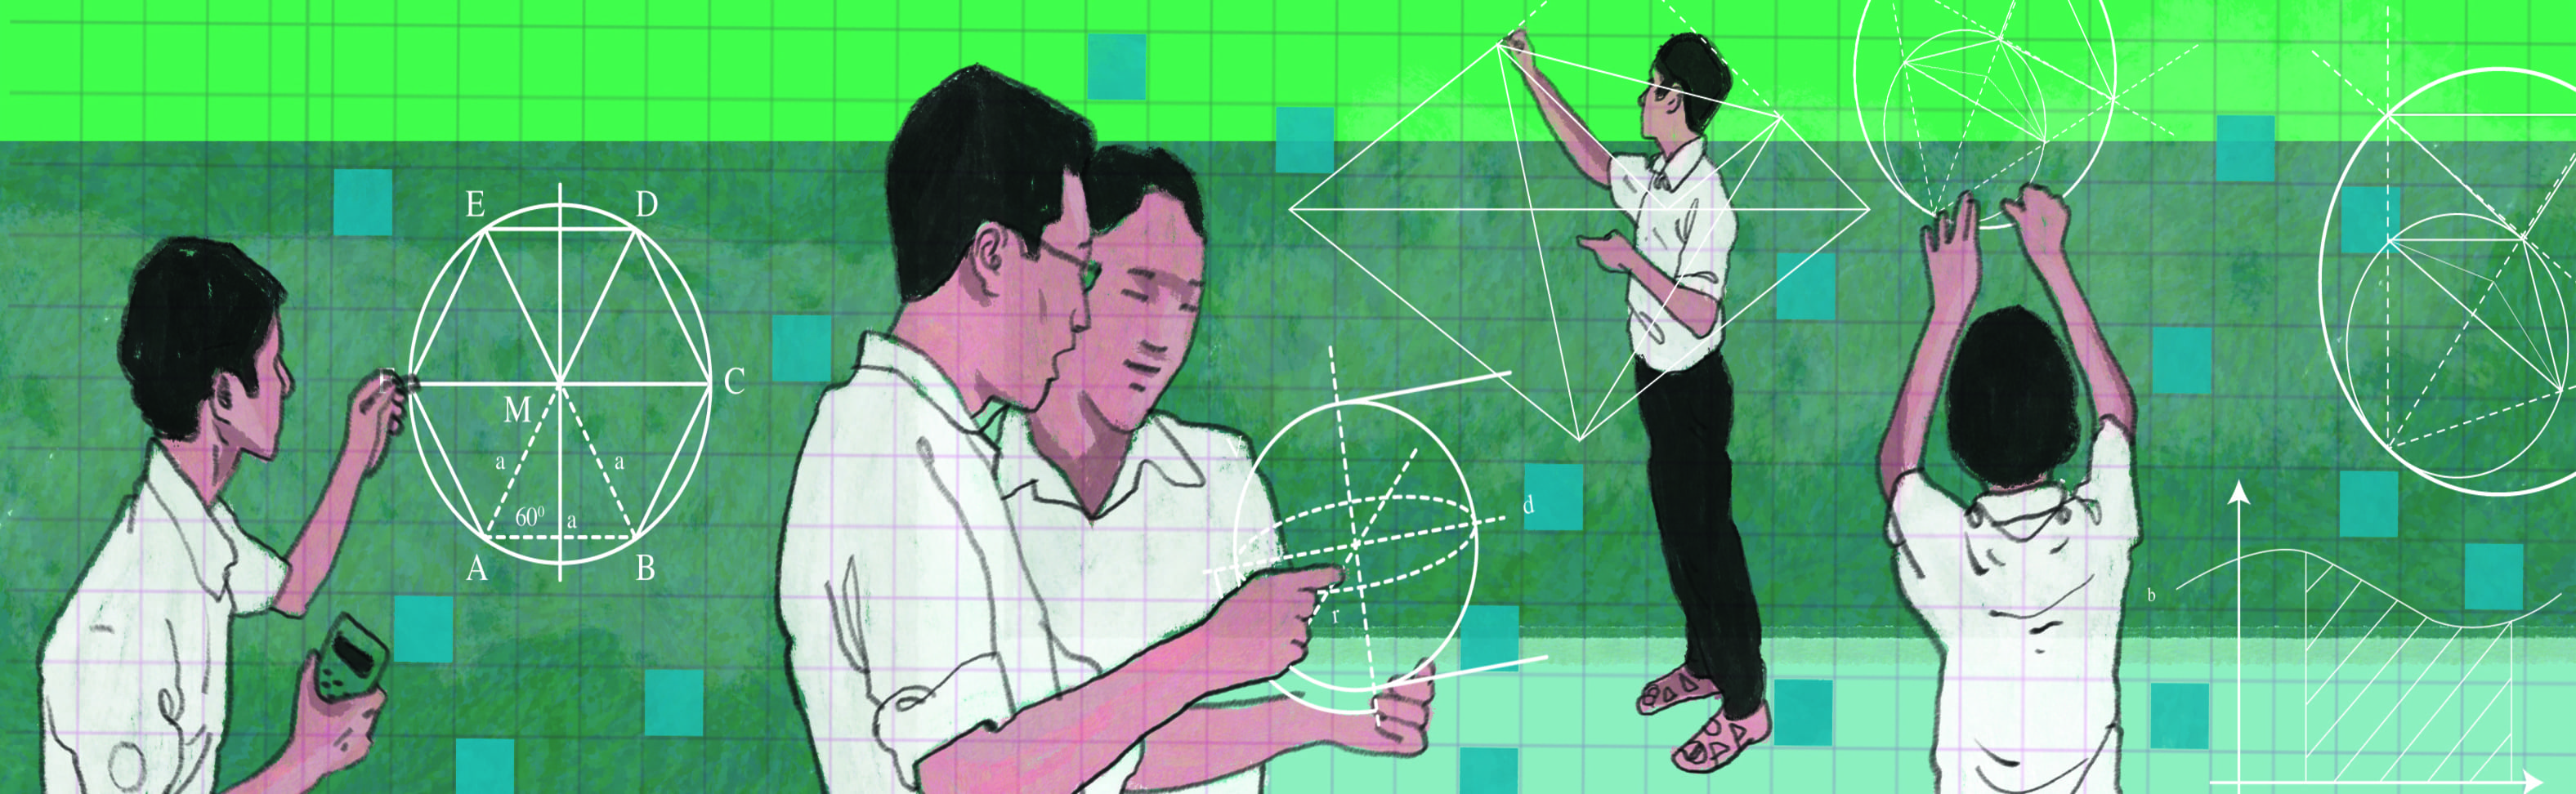
\includegraphics[width=19.3cm]{../bannerdiendan}}}
\AddToShipoutPicture*{\put(56,530){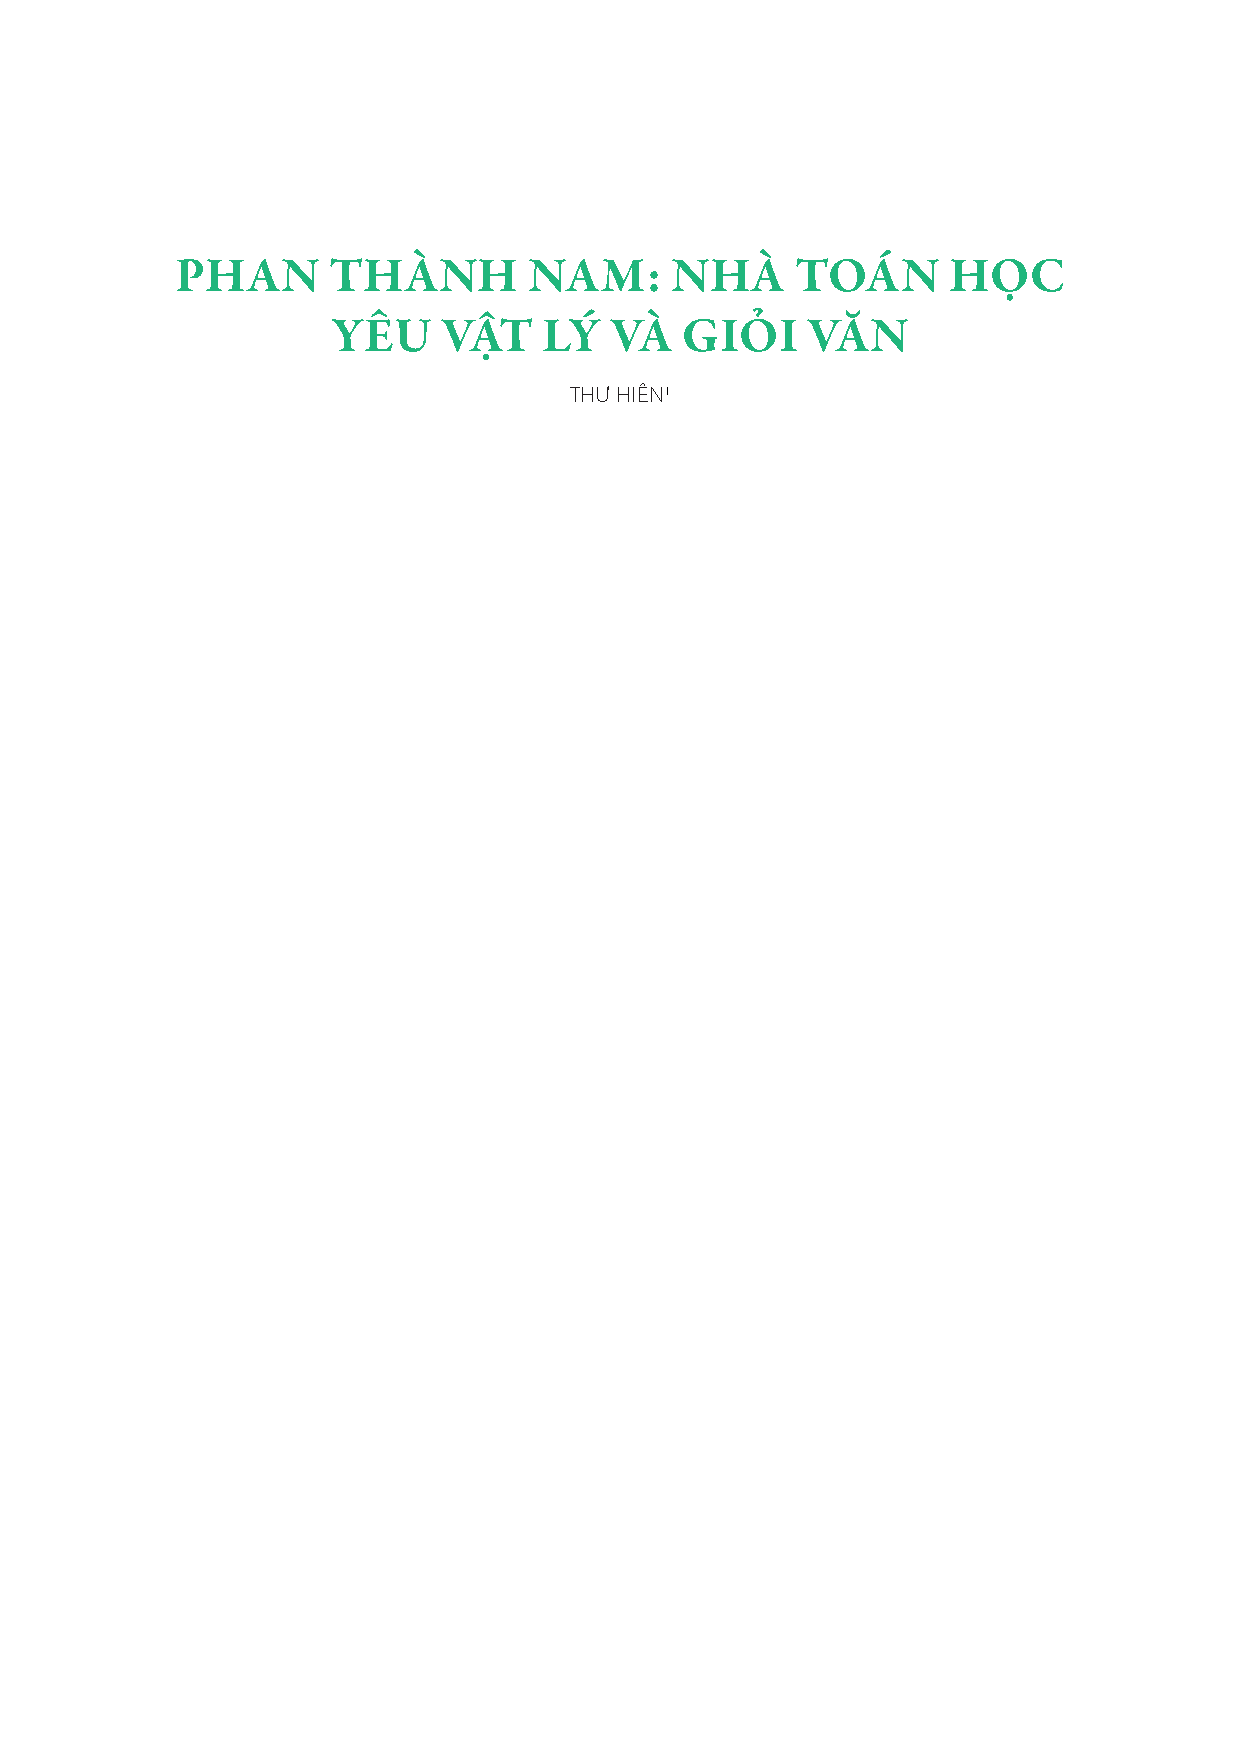
\includegraphics[scale=1]{../tieude.pdf}}}
\centering
\endgroup
\vspace*{182pt}

\textit{\textbf{\color{diendantoanhoc}LTS.} Phan Thành Nam dành giải thưởng của Hội toán học châu Âu năm $2020$. Giải thưởng này được trao bốn năm một lần trong Đại hội Toán học Châu Âu (ECM) cho các nhà khoa học trẻ (không quá $35$ tuổi) nhằm ghi nhận những đóng góp xuất sắc trong lĩnh vực toán học. Nhân dịp Phan Thành Nam về công tác tại Việt Nam, anh đã có những chia sẻ với Pi về con đường học tập của mình.}
\begin{multicols}{2}
	Dù ẵm giải nhì học sinh giỏi văn cấp tỉnh dành cho học sinh THCS nhưng cậu học trò Phan Thành Nam lại ước mơ trở thành nhà vật lý. Vậy là anh quyết tâm thi chuyên toán vì nghe nói muốn hiểu vật lý thì phải giỏi toán. Giấc mơ thưở thiếu thời đó đã dẫn dắt anh đến với giải thưởng chính của Hội toán học châu Âu EMS, bởi những thành tựu dùng toán để giải quyết các vấn đề vật lý lượng tử~...
	\begin{figure}[H]
		\centering
		\vspace*{-5pt}
		\captionsetup{labelformat= empty, justification=centering}
		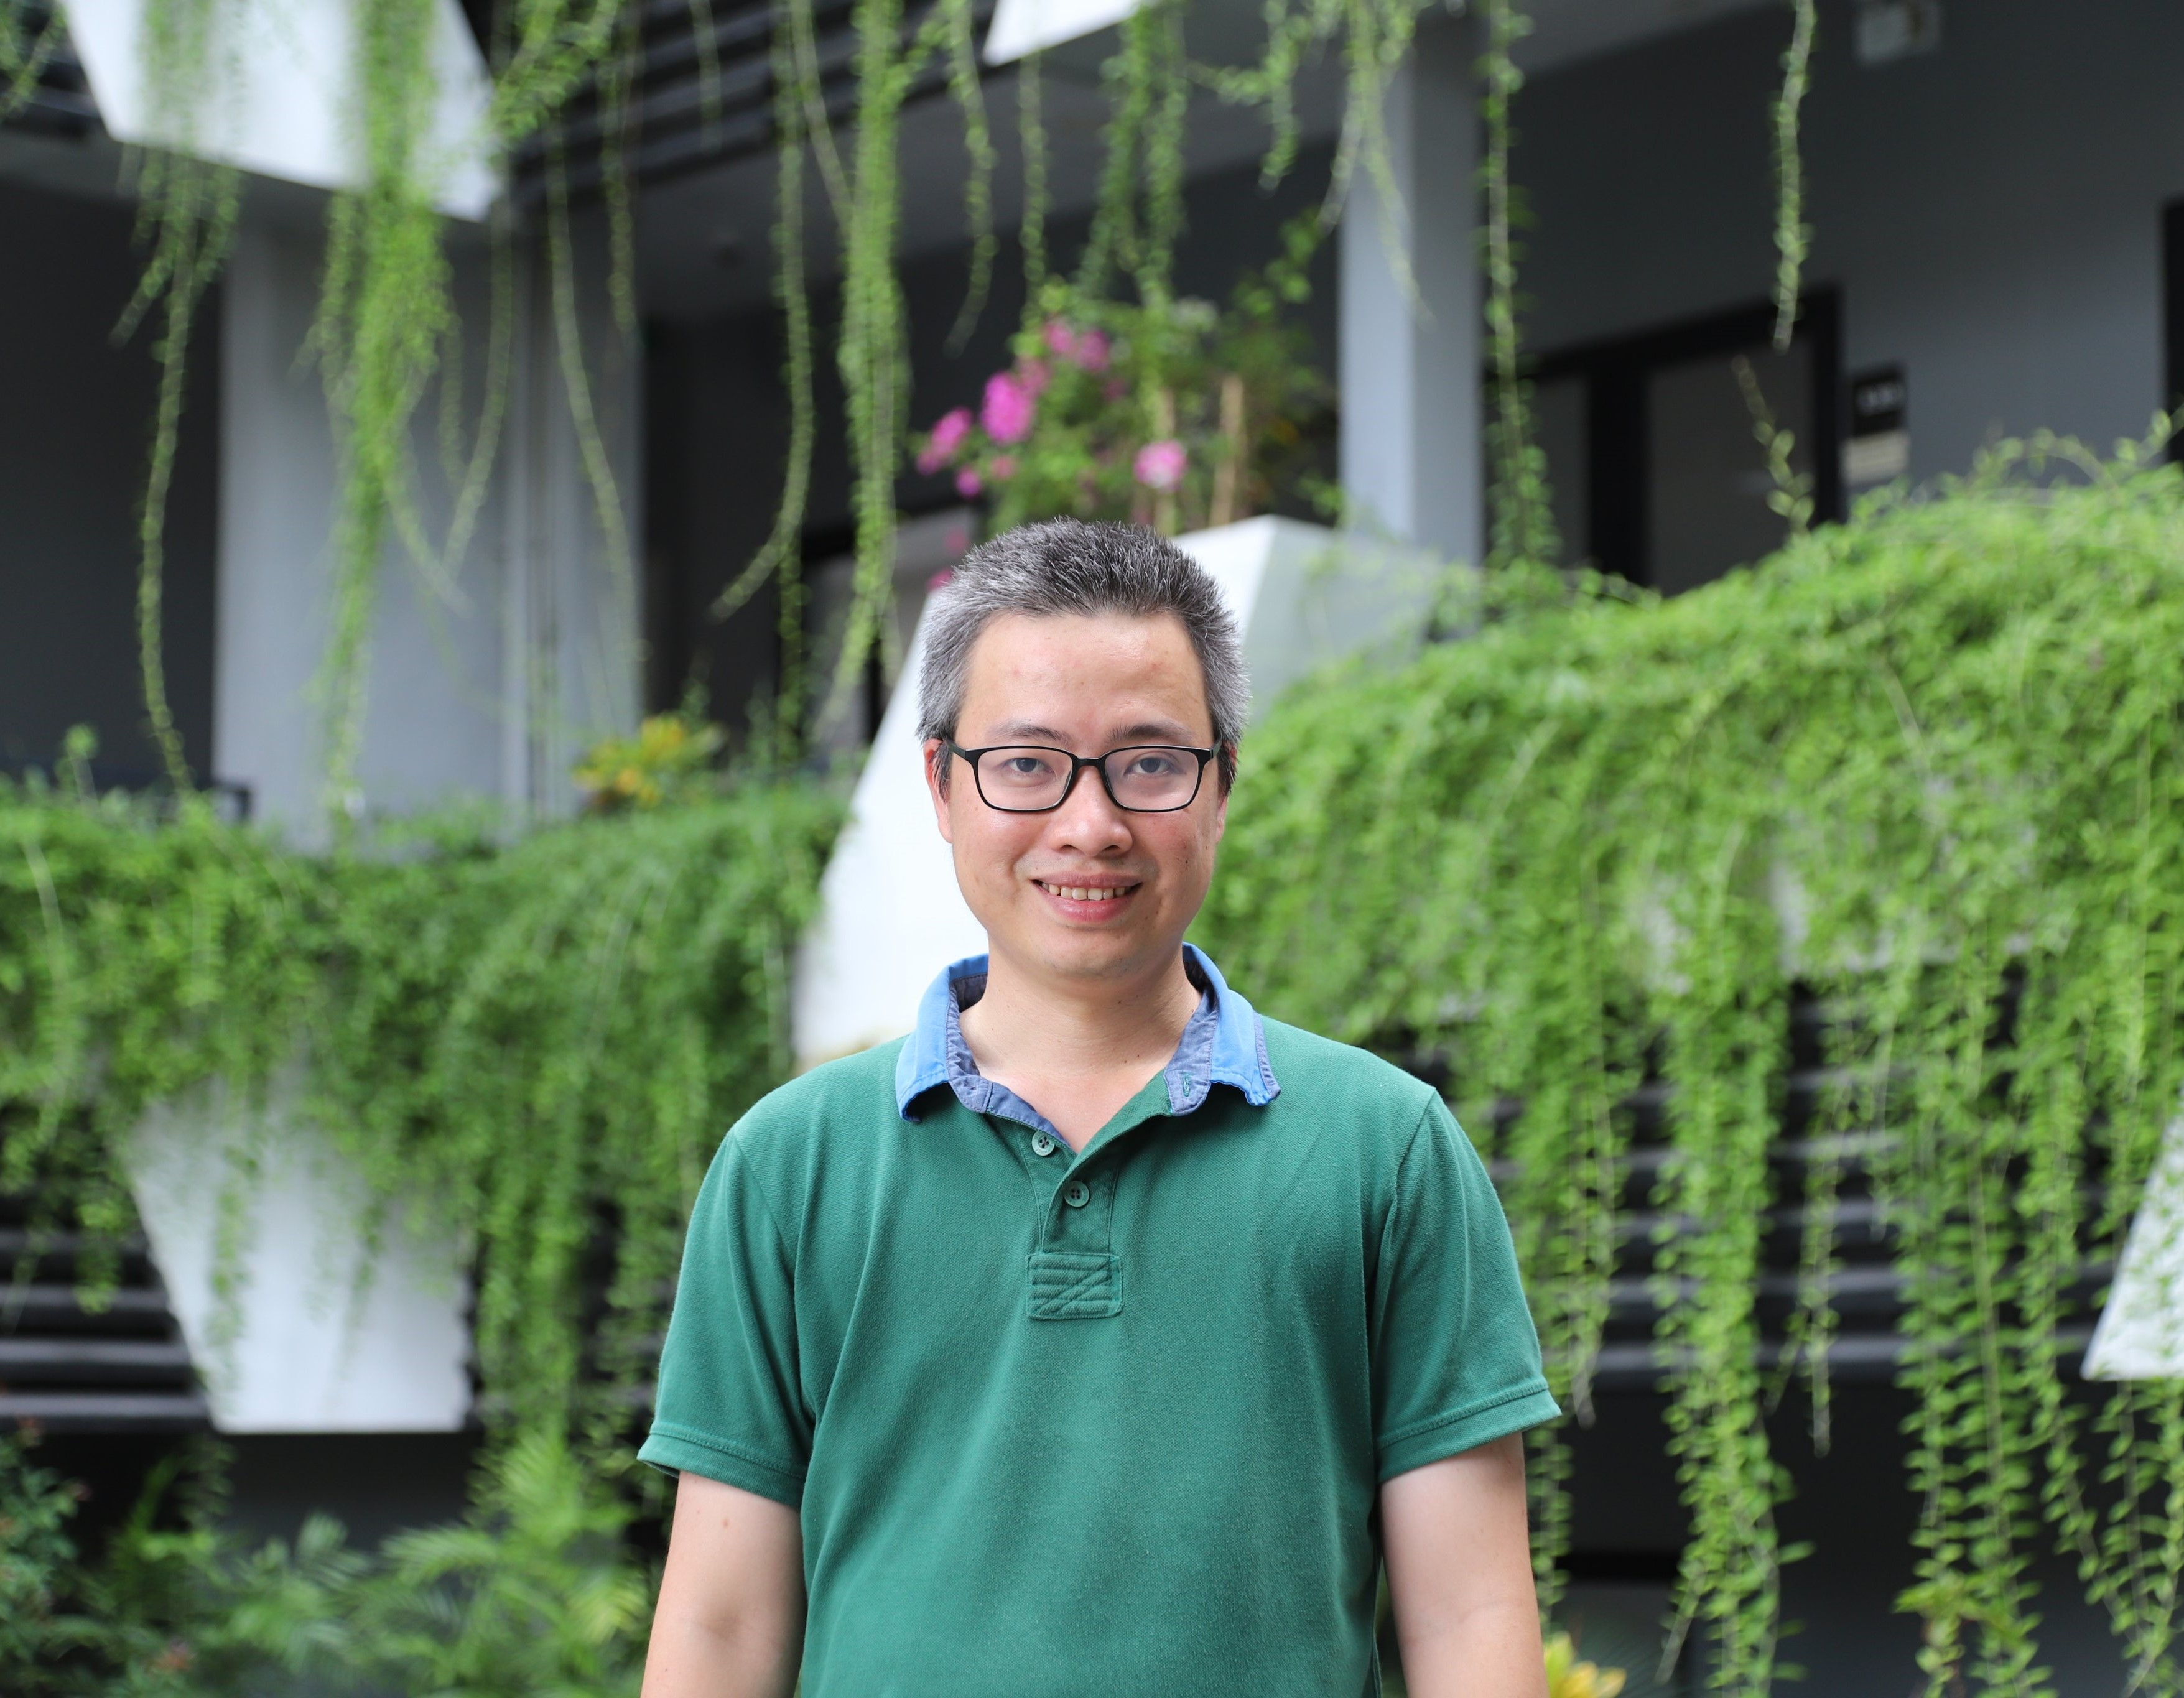
\includegraphics[width=1\linewidth]{1}
		\caption{\small\textit{\color{diendantoanhoc}GS. Phan Thành Nam tại Viện nghiên cứu cao cấp về Toán. Ảnh: Quang Huy.}}
		\vspace*{-10pt}
	\end{figure}
	\textbf{\color{diendantoanhoc}Ước mơ khởi đầu: trở thành nhà vật lý}
	\vskip 0.1cm
	\textit{Xin chào Phan Thành Nam, anh có thể chia sẻ với Pi về hành trình dẫn anh đến với toán học? Hẳn là anh đã từng là học sinh chuyên toán từ nhỏ, vào ĐH cũng học toán?}
	\vskip 0.1cm
	Đúng là hồi lớp $6$ thì tôi học chuyên toán trường Lương Văn Chánh ở Phú Yên. Gọi là lớp chuyên toán nhưng cũng chỉ khác lớp thường là mỗi tuần chúng tôi được bồi dưỡng thêm vài buổi với nội dung học vượt ra ngoài sách giáo khoa, còn giờ học chính khóa thì cũng học như các bạn lớp thường. Nhưng sau đó mô hình chuyên cấp THCS không còn, lên lớp $7$ tôi trở về học lớp thường. Tôi học đều và thích nhiều môn, năm lớp $9$ còn được giải nhì học sinh giỏi cấp tỉnh môn văn.
	\vskip 0.1cm
	\textit{Ơ, sao tự nhiên anh lại đi thi học sinh giỏi môn văn?}
	\vskip 0.1cm 
	Ban đầu tôi thi học sinh giỏi toán, nhưng bị trượt, không được chọn vào đội tuyển của trường để đi thi tiếp. Vì thế mà cô giáo dạy văn khích lệ tôi thi học sinh giỏi môn văn. Tôi thấy đây là một gợi ý hay, môn văn là môn ``truyền thống" của gia đình tôi, mẹ tôi là giáo viên văn, ba tôi vốn học cử nhân văn ở Trường ĐH Tổng  hợp Huế và sau này làm nhà báo. Trong nhà tôi có rất nhiều sách văn học, lúc rảnh rỗi tôi đọc hết nên cũng rất thích môn văn.  
	\vskip 0.1cm
	\textit{Giải nhì văn cấp tỉnh là một thành tựu ngọt ngào, sao anh không tiếp tục đầu tư cho môn văn mà lại trở thành nhà toán học?}
	\vskip 0.1cm 
	Thật ra khi đó tôi lại ôm ấp một giấc mơ khác, đó là trở thành nhà vật lý. Ấy là do ảnh hưởng của cuốn sách \textbf{\color{diendantoanhoc}\textit{``Các nhà vật lý đi tiên phong"}}, mà hồi đó tôi vừa đọc xong. Tuy nhiên trong sách đó viết rằng để hiểu vật lý thì phải giỏi toán, nên khi vào cấp $3$, tôi chọn thi vào lớp chuyên toán ở Trường THPT chuyên Lương Văn Chánh. 
	\vskip 0.1cm
	\textit{Thi vào đội tuyển toán của trường THCS mà còn bị trượt, vậy mà lại tiếp tục mơ mộng thi vào chuyên toán trường chuyên của tỉnh. Xem ra anh cũng ``liều"?} 
	\vskip 0.1cm
	Đúng là có một chút liều. Nhưng vì nhờ việc trượt đội tuyển toán ở lớp $9$ mà tôi nhận ra mình còn thiếu kiến thức nào để bổ sung trong quá trình ôn thi vào lớp $10$ chuyên toán sau này. Trước đó tôi gần như không học nội dung gì ngoài SGK. Khi ôn thi chuyên toán, tôi mới bắt đầu đào sâu một số nội dung ngoài SGK.
	\vskip 0.1cm
	Thật may là tôi đã đỗ chuyên toán, tuy với mức điểm trung bình nhưng đó là một sự khởi đầu tuyệt vời bởi từ đó tôi được học các thầy dạy toán rất giỏi, họ gieo vào tôi tình yêu, niềm đam mê với toán. 
	\vskip 0.1cm
	\textbf{\color{diendantoanhoc}Học để thỏa mãn đam mê chứ không vì thi thố}
	\vskip 0.1cm
	\textit{Đỗ chuyên toán với mức điểm trung bình, vậy việc học sau đó của anh có chật vật để theo kịp các bạn trong lớp không?}
	\vskip 0.1cm
	Tôi thấy việc học cũng nhẹ nhàng. Cuối năm lớp $10$ tôi còn được chọn đi dự kỳ thi Olympic $30.4$, nhờ đó mà tôi được giao lưu với các bạn học sinh giỏi toán các địa phương khác. Chúng ta vẫn nói về tầm quan trọng của việc được học với các thầy giỏi, nhưng từ trải nghiệm của chính mình, tôi thấy việc được học chung với các bạn giỏi cũng quan trọng không kém. 
	\vskip 0.1cm
	Hồi đó lớp tôi có một bạn rất giỏi, tên là Phùng Trọng Thực (hiện là GV Trường ĐH Bách khoa TP.HCM). Có lần Thực đưa cho tôi một bài toán rất hay và lạ, hỏi có giải được không? Thực cho biết bài toán đó có trong tờ tạp chí Toán học và Tuổi trẻ, đây là lần đầu tôi biết tới tạp chí này. Từ đó, $2$ đứa cùng có thêm một niềm vui chung là ngóng chờ tạp chí \textbf{\color{diendantoanhoc}\textit{Toán học và Tuổi trẻ}} về hàng tháng để ngồi giải bài. Chúng tôi áng chừng thời gian tạp chí về đến Phú Yên (thường chậm hơn thời điểm phát hành ở Hà Nội vài ngày), những ngày đó lảng vảng quanh bưu điện liên tục để hễ tạp chí về đến nơi là mua được ngay. 
	\vskip 0.1cm
	Thời gian đầu, gần như chúng tôi chẳng giải được bài toán nào đăng trong tạp chí đó. Lúc đó chúng tôi mới vào lớp $10$, nhưng có nhiều bài thuộc chương trình lớp $11-12$, nên chúng tôi tự học các kiến thức liên quan trong SGK các lớp trên để có đủ nền tảng cần thiết. Nhờ sự ``máu mê" đó mà chúng tôi bắt đầu giải được bài đầu tiên, rồi bài thứ  hai, thứ ba ...
	\vskip 0.1cm 
	Lên lớp $11$ thì tôi đạt giải nhì HSG quốc gia, được ra Hà Nội thi chọn đội tuyển quốc tế. Có khoảng $40$ bạn dự thi, để chọn ra $6$ bạn. Đề thi rất khó, có những dạng toán tôi chưa gặp bao giờ. Tôi nhớ một kỷ niệm vui là nhờ được mang đồ ăn vào phòng thi, mà tôi có việc để làm lúc thi, tức là tôi chủ yếu ngồi ăn chứ toán thì không làm được bao nhiêu.  
	\vskip 0.1cm
	Lớp $12$ tôi cũng được đi thi quốc gia, nhưng chỉ đạt giải khuyến khích. Lúc đó tôi cảm thấy rất tự tin, vì đã học thêm được rất nhiều kiến thức so với năm lớp $11$, nhưng khi vào phòng thi lại làm bài không tốt.  
	\vskip 0.1cm
	\textit{Không được ``hái quả ngọt" vào năm học lớp $12$ mà anh không nản lòng à, để lại vẫn tiếp tục học toán khi lên ĐH?}   
	\vskip 0.1cm
	Lúc đó tình yêu toán đã bén rễ sâu đậm trong tôi, tôi học là để thỏa mãn đam mê chứ không phải để thi thố. 
	\vskip 0.1cm
	Nhờ đạt giải học sinh giỏi quốc gia, tôi được tuyển thẳng vào ĐH. Lúc đó tôi có nhiều lựa chọn. Ngành CNTT của Trường ĐH Bách khoa TP.HCM là ngành thời thượng. Các trường y dược cũng là mục tiêu phấn đấu của nhiều bạn học sinh giỏi. Còn khoa toán tin Trường ĐH Khoa học tự nhiên, ĐH Quốc gia TP.HCM có điểm chuẩn rất thấp, khoảng $15$ điểm/$3$ môn là đỗ. Tuy nhiên tôi chẳng bận tâm, vì thích toán quá rồi, cứ được học toán tiếp là tôi học. 
	\vskip 0.1cm
	Lúc đó tôi rất thích cuốn sách \textbf{\color{diendantoanhoc}\textit{``Tìm tòi để học giỏi toán"}} của anh Lê Quang Nẫm. Biết anh Nẫm là sinh viên Trường ĐH Khoa học tự nhiên, ĐH Quốc gia TP.HCM, tôi muốn vào đó học, với hy vọng có cơ hội được gặp anh, hoặc được học với các thầy của anh. 
	\vskip 0.1cm
	Anh Lê Quang Nẫm hơn tôi khoảng $5$ tuổi, lúc là học sinh đã rất nổi tiếng. Anh là con nhà nghèo, khi anh trúng tuyển vào lớp $10$ Trường Phổ thông Năng khiếu của ĐH Quốc gia TP.HCM thì ba của anh phải từ Quảng Ngãi vào TP.HCM để đạp xích lô nuôi anh ăn học. Học xong cấp $3$ anh vào khoa Toán tin Trường ĐH Khoa học tự nhiên, và tốt nghiệp thủ khoa. Nhưng đó là những thông tin về sau tôi mới biết. Còn khi đọc cuốn sách của anh Nẫm tôi cảm thấy ngưỡng mộ vì anh viết hấp dẫn quá. 
	\vskip 0.1cm
	\textit{Ba mẹ anh có ý kiến thế nào khi anh chọn học toán?}
	\vskip 0.1cm 
	Ba mẹ tôi dân chủ lắm, chỉ cung cấp thông tin về một số trường/ngành mà ba mẹ nghĩ là tốt, còn quyết định là do tôi. Thật sự lúc đó tôi cũng không mường tượng con đường học Toán ở ĐHKHTN TPHCM là như thế nào. Tôi chỉ nghĩ là có thể nó sẽ giúp mình trở thành giáo viên dạy toán, mà như thế cũng tốt. Thời đó sinh viên tốt nghiệp các ngành khoa học cơ bản mà có chứng chỉ sư phạm là cũng được dạy phổ thông. 
	\vskip 0.1cm
	Đó là một quyết định sáng suốt. Vì khi vào học đại học thì tôi rất may mắn gặp được các thầy giỏi, tâm huyết. Thầy này giúp tôi đến với thầy khác, nhờ thế mà hành trình giúp tôi đến với toán học khá suôn sẻ. 
	\vskip 0.1cm
	\textbf{\color{diendantoanhoc}Dùng toán để hiểu vật lý và khám phá thế giới}
	\vskip 0.1cm 
	\textit{Anh được Hội toán học châu Âu trao giải thưởng chính là bởi thành tựu nào trong nghiên cứu toán học của anh?}
	\vskip 0.1cm 
	Họ xét giải trên cơ sở một cụm công trình, cụ thể là ghi nhận đóng góp của tôi cho lĩnh vực vật lý lượng tử đa hạt. Thông thường trong vật lý lượng tử, để biết tính chất của một hệ thì mình phải giải một phương trình Schrödinger (phương trình đươc đặt theo tên nhà vật lý học người Áo, người đầu tiên thiết lập phương trình này và được giải Nobel vật lý năm $1933$). Nếu hệ chỉ có một hạt, thì phương trình Schrödinger chỉ có một biến trong không gian ba chiều. Nếu hệ có $N$ hạt thì phương trình có $N$ biến, và trong nhiều ứng dụng số lượng biến số rất lớn tới mức mình không thể giải được, kể cả giải chính xác hoặc giải số bằng máy tính. 
	\vskip 0.1cm
	%	\begin{figure}[H]
		%		\centering
		%		\vspace*{-5pt}
		%		\captionsetup{labelformat= empty, justification=centering}
		%		
\includegraphics[width=1\linewidth]{3}
		%		\caption{\small\textit{\color{diendantoanhoc}GS. Phan Thành Nam và một sinh viên. Anh: Quang Huy.}}
		%		\vspace*{-10pt}
		%	\end{figure}
	Vì đó là một bài toán rất phức tạp, mình cần sẽ tiếp cận bằng các phương pháp xấp xỉ, thường là thay phương trình tuyến tính nhiều biến bằng phương trình phi tuyến một biến. Đây là phương pháp mà các nhà vật lý học đã phát triển trong một thời gian dài. Câu hỏi đặt ra là làm sao chứng minh được phương pháp xấp xỉ đó là đúng, nghĩa là khi số hạt N tiến về vô cùng thì mô hình xấp xỉ trở thành chính xác. Bằng cách sử dụng và phát triển các công cụ trong toán giải tích, tôi chứng minh được rằng trong những điều kiện cụ thể thì một số mô hình xấp xỉ sẽ đúng với những nguyên lý căn bản trong cơ học lượng tử. 
	\vskip 0.1cm
	\textit{Ở trên anh kể chuyện hồi lớp $9$ anh từng mơ ước trở thành nhà vật lý nên nên mới cố gắng học giỏi toán. Vậy việc sau này anh chọn nghiên cứu sâu về toán trong vật lý lượng tử, việc này có liên quan gì tới ước mơ hồi đó?}
	\vskip 0.1cm 
	Đúng là có liên quan. Sau khi làm thạc sĩ, tôi xin được một số học bổng tiến sĩ khác nhau, có cả toán lý thuyết và toán ứng dụng. Tình cờ trong thời gian này, tôi đọc một cuốn sách rất thú vị là \textbf{\color{diendantoanhoc}\textit{``Lưới trời ai dệt"}} của tác giả Nguyễn Tường Bách. Trong cuốn đó, tác giả trình bày về vật lý lượng tử một cách rất cuốn hút, với nhiều mối liên quan tới triết học Phật giáo. Điều này làm sống lại uớc mơ hồi năm lớp $9$, vốn vẫn quanh quẩn trong tâm trí tôi, đó là học về Vật lý Toán.  
	\vskip 0.1cm
	Vì thế mà tôi chọn GS Jan Philip Solovej ở ĐH Copenhaghen để xin học lên tiến sĩ. Khi đó, tôi vào trang khoa toán tìm các giáo sư, và cảm thấy các công trình nghiên cứu của GS Solovej về vật lý lượng tử là vô cùng hấp dẫn. Mặc dù tôi không hiểu rõ các công trình đó, nhưng cảm thấy các kiến thức toán này nếu cố gắng mình sẽ học được, nên quyết định xin theo thầy. Tôi rất may mắn là được thầy đồng ý. 
	\vskip 0.1cm
	Tôi nghĩ môn vật lý ở chương trình phổ thông là một môn học thú vị, nó giúp cho những đứa trẻ thỏa mãn sự tò mò khi tìm hiểu các hiện tượng tự nhiên. Sau này, nhờ sử dụng các công cụ bên toán mà tôi hiểu được chính xác các khái niệm vật lý, điều này kiến tôi thấy rất sung sướng. Mặc dù có thể đó là những điều nhân loại hiểu ra từ cách đây hàng trăm năm, nhưng khi được đi lại trên con đường khám phá thế giới mà nhân loại đã từng đi, tôi vẫn thấy thật hạnh phúc. 
	\vskip 0.1cm
	\textbf{\color{diendantoanhoc}Sẽ cùng các đồng nghiệp người Việt ở nước ngoài giúp VN lấp khoảng trống vật lý toán...}
	\vskip 0.1cm
	\textit{Anh có biết, ở Việt Nam, có những ai làm việc trong lĩnh vực nghiên cứu của anh không?}
	\vskip 0.1cm 
	Tôi gần như không biết có ai làm về lĩnh vực này ở VN! Có một số nhóm vật lý lý thuyết làm việc trực tiếp với những mô hình xấp xỉ phi tuyến, và một số nhóm vật lý thực nghiệm kiểm tra các mô hình xấp xỉ đó có đúng hay không. Nhưng có vẻ như không có nhà toán học nào nghiên cứu những phương trình nhiều hạt từ các nguyên lý cơ \linebreak bản nhất.  
	\vskip 0.1cm
	\textit{Có nghĩa là lĩnh vực này đang có một khoảng trống lớn ở VN?}
	\vskip 0.1cm 
	Vâng, đúng rồi. Nhưng tôi nghĩ tôi có thời gian để giúp cải thiện việc này. 
	\vskip 0.1cm
	Đầu tháng $8$ vừa rồi, tôi cùng anh Nguyễn Trọng Toán (GS ở ĐH bang Pennsylvania, Mỹ) tổ chức một trường hè về vật lý toán bên Viện Nghiên cứu cao cấp về Toán (nơi GS Ngô Bảo Châu là Giám đốc khoa học -- PV). Chúng tôi bất ngờ trước sự say mê học hỏi của các bạn trẻ. Trong cả buổi sáng họ nghe chúng tôi giảng bài, tới buổi chiều vẫn kiên trì ngồi lại lớp học làm bài tập. Sau đó tôi dự hội thảo về phương trình đạo hàm riêng kỷ niệm ngày sinh GS Đinh Nho Hào ở Viện toán học VN. Tôi thấy nhiều báo cáo đạt chất lượng rất cao, ngang tầm chất lượng các hội thảo đẳng cấp quốc tế. Điều đặc biệt là có nhiều báo cáo của các bạn trẻ. Do đó, tôi thấy rất lạc quan với sự phát triển của ngành này ở trong nước, và trước mắt tôi có thể dùng các công cụ của ngành phương trình đạo hàm riêng để tương tác với các nhà toán học trong nước. 
	\vskip 0.1cm
	%	\begin{figure}[H]
		%		\centering
		%		\vspace*{5pt}
		%		\captionsetup{labelformat= empty, justification=centering}
		%		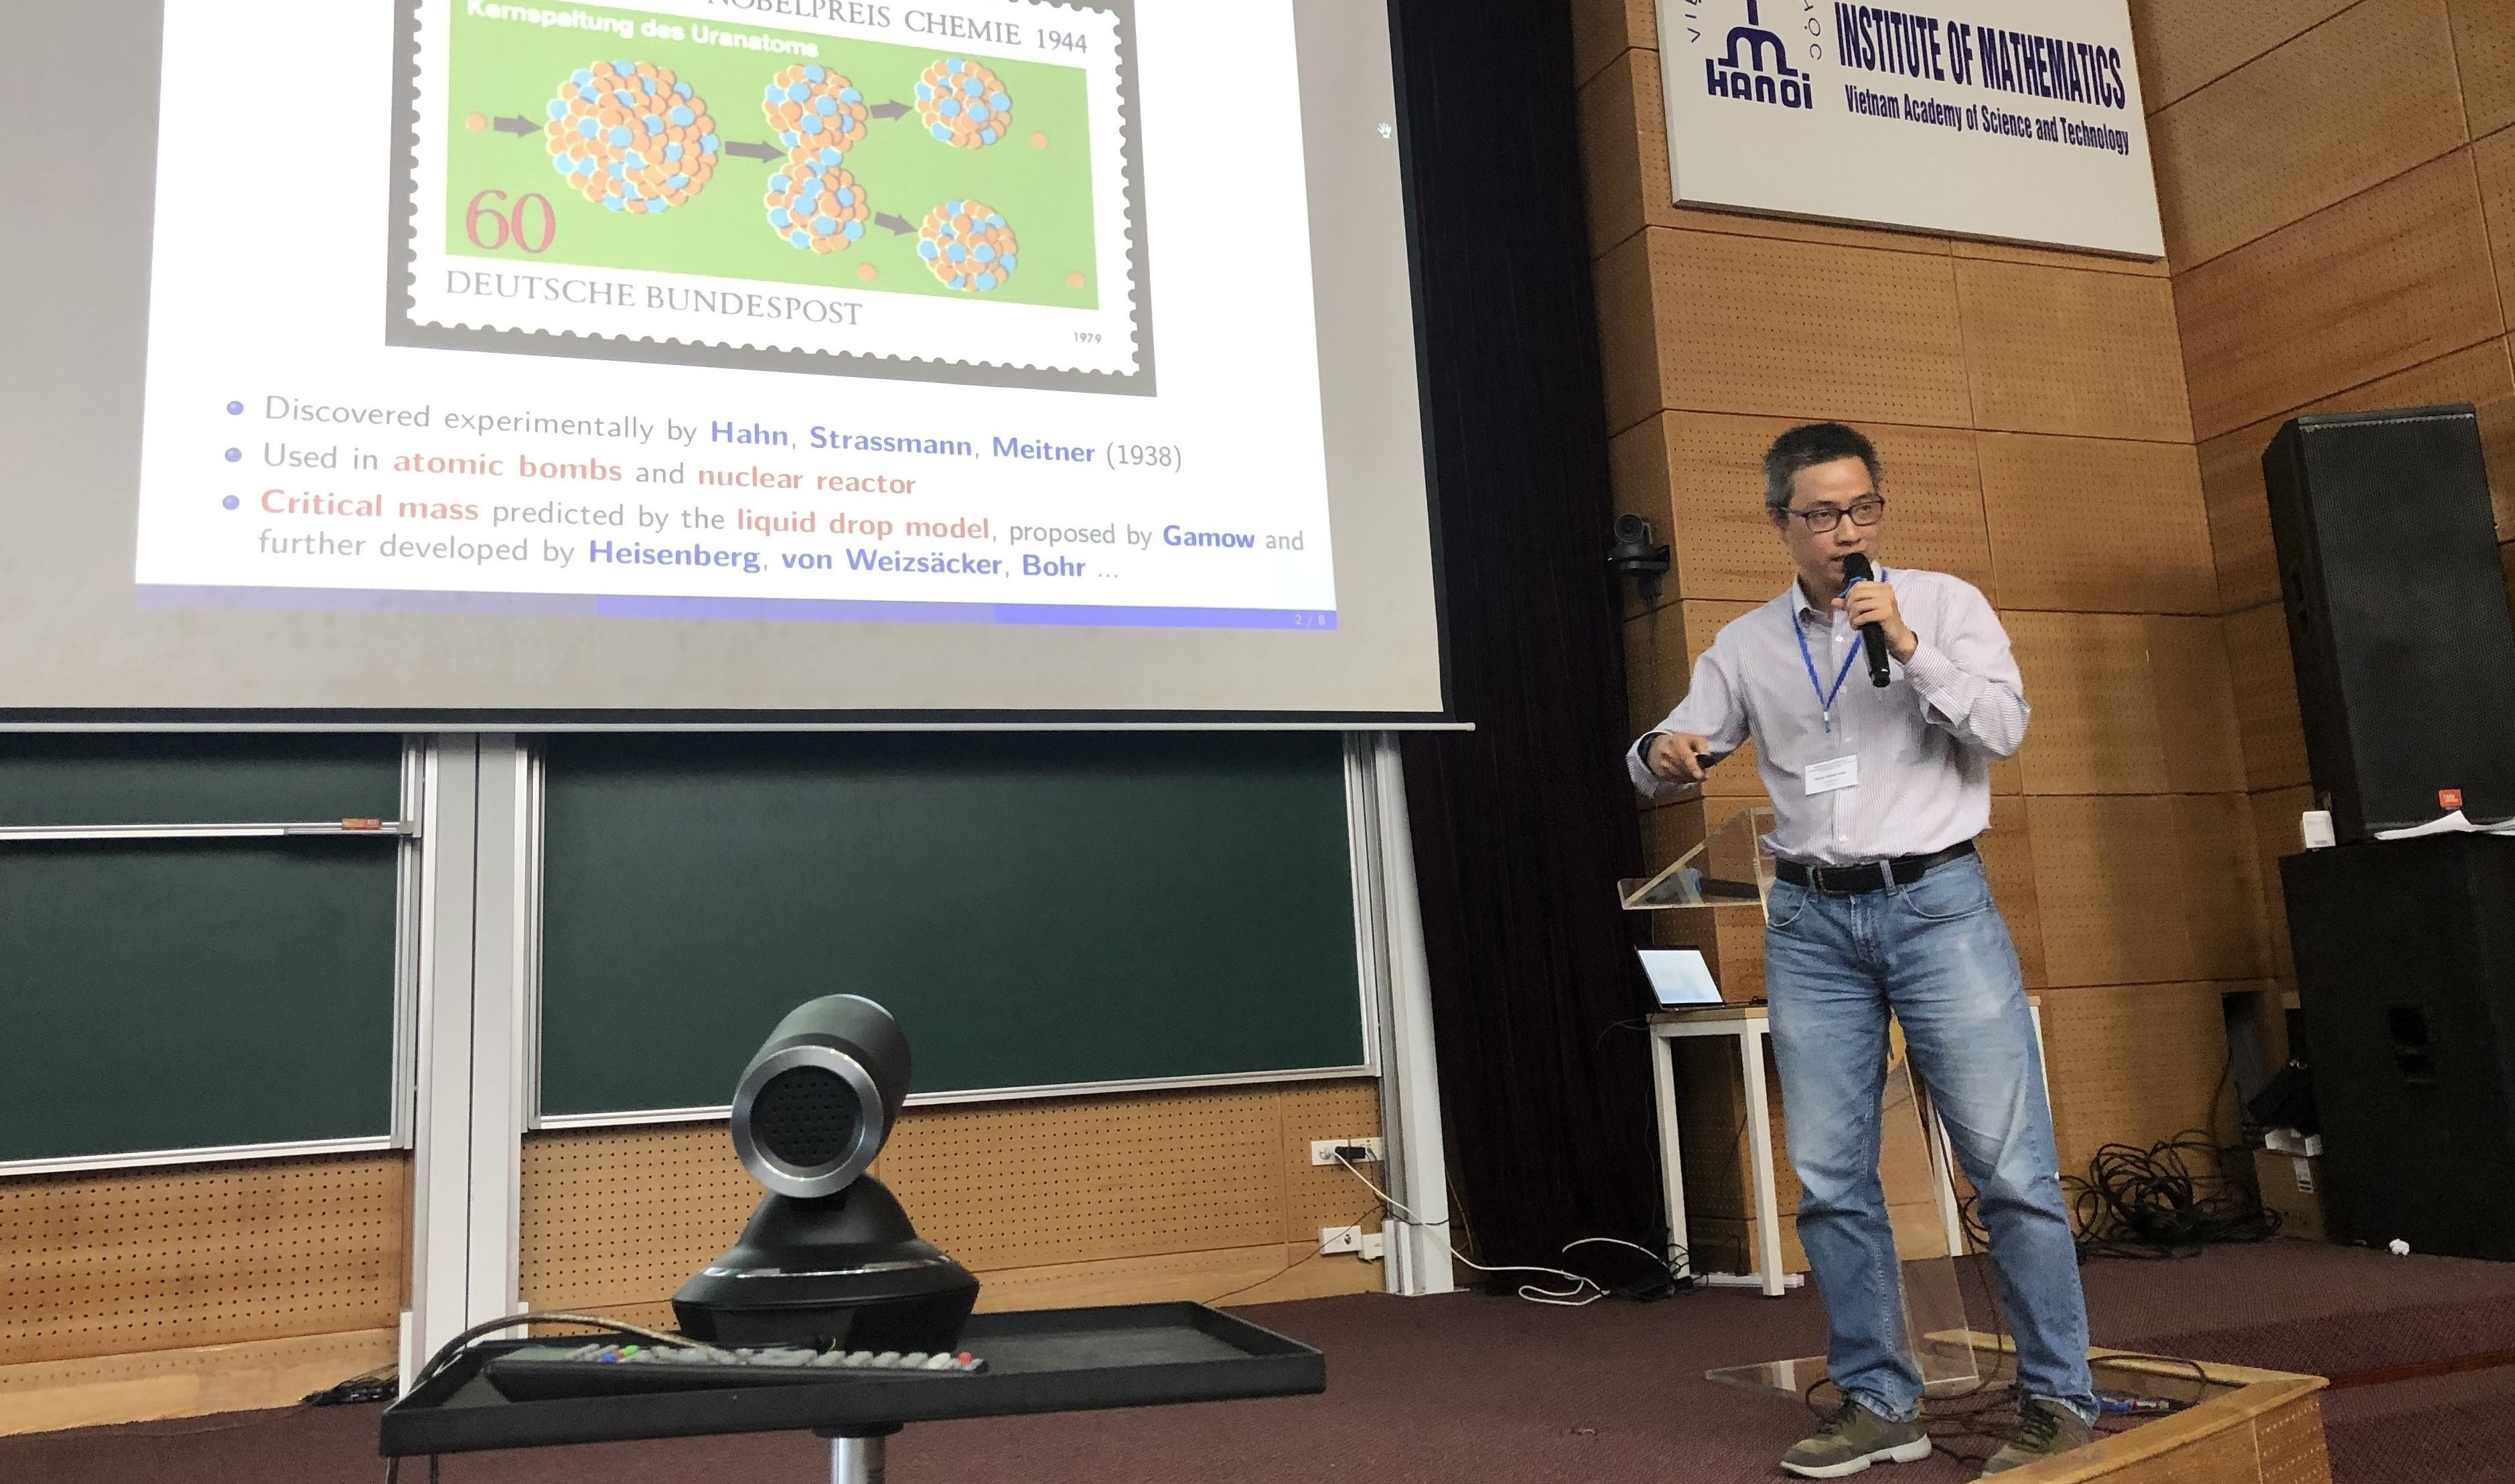
\includegraphics[width=1\linewidth]{4}
		%		\caption{\small\textit{\color{diendantoanhoc}GS. Phan Thành Nam báo cáo tại Viện Toán học. Ảnh: Viện Toán học.}}
		%		\vspace*{-10pt}
		%	\end{figure}
	Để xây dựng ngành của mình ở VN, tôi cần phải tiếp tục tổ chức một số trường hè, tổ chức dạy học một số môn học trong các khoa toán của các trường ĐH. Tôi đã trao đổi với một số nhà toán học trong nước và được các anh ủng hộ. Trước hết các thầy trong nước sẽ dạy trước cho sinh viên một số kiến thức tổng quát, sau đó tôi sẽ dạy phần tiếp theo, đi sâu hơn vào lĩnh vực nghiên cứu hiện đại. Bằng các giải pháp đồng thời như trên, tôi hy vọng sẽ có một số bạn trẻ sẽ nảy sinh đam mê về vật lý toán.
	\vskip 0.1cm 
	Một thuận lợi là với riêng ngành giải tích -- phương trình đạo hàm riêng, tôi có nhiều ``đồng minh" là các anh chị người Việt xuất thân từ trường ĐH Khoa học tự nhiên, ĐH Quốc gia TP.HCM và đã đạt được vị trí vững vàng trong các trường đại học hàng đầu trên thế giới. Ở Châu Âu có anh Nguyễn Hoài Minh (GS ĐH Paris Sorbonne ở Pháp); anh Nguyễn Lê Lực (GS ĐH ở Anh); anh Trương Trung Tuyến (GS ĐH Oslo, Na Uy). Ở Mỹ có anh  Nguyễn Trọng Toán (GS ĐH bang Pennsylvania), anh Lê Quang Nẫm (GS ĐH Indiana), anh Trần Vĩnh Hưng (GS ĐH Wisconsin–Madison), anh Phan Văn  Tuộc (GS ĐH Tennessee), anh Trần Minh Bình (GS ĐH Texas A\&M) ... và rất nhiều anh chị khác. Đó là những người trẻ trên dưới $40$ tuổi, đang làm việc rất tích cực, và mọi người đều đồng lòng hướng về VN với mong muốn tham gia vào sự phát triển toán học trong nước.
	\vskip 0.1cm
	\textit{Xin cảm ơn GS Phan Thành Nam!} 
\end{multicols}